% comparamos implemtaciones del mismo filtro (versión mas intuitiva posible de c vs asm con SIMD). Esto permite analizar mejor la optimizaciones del compilador. Sobre todo las de icc que tiene introducción automática de SIMD
% En todos los casos se realizó el gráfico C vs ASM (cantidad de clocks y cantidad de líneas de código).
% Como medimos. (menor vs promedio)
% Como se compiló. Compilamos con gcc, con icc, y con diferentes flags.
	% - (aclarar cuales y por qué)
	% - Explicar por qué se puso ICC y no otro(introduce SIMD automáticamente y se supone que es el compilador mas optimo para la arquitectura AMD-64 con procesadores intel).
% cómo se ejcutó. (Mínimas interrupciones, init 2 y kill -9 -1).
% Análisis del código. (object dump).
% - Los tres filtros se programaron pensando en minizar los accesos a memoria incluso en situaciones donde producía cálculo extra.

	A la hora de implementar los filtros se tuvieron algunas consideraciones generales 
para poder explicar los resultados de manera correcta, para manetener la coherencia
interna dentro del trabajo y para tener bases firmes en las que basarnos para sacar
conclusiones.

\subsection{Criterios de implementación}

\begin{itemize}
			\item Todas las implementaciones de C intentan ser lo mas intuitivas posibles. No se
			utilizaron optimizaciones demasiado extrañas. Intentan ser una traducción bastante
			fiel de la descripción en lenguaje natural del enunciado a C. Decimos esto para
			poder analizar de manera pura la diferencia entre los dos paradigmas. Además
			a la hora de analizar los archivos objeto creados por los compiladores
			tener un algorítmo simple ayuda a hacer un análisi mas simple y consistente.
			Por otra parte da libertad al compilador para meter tanta paralelización como pueda
			de tal manera que los diferentes compiladores puedan introducir ellos las optimizaciones
			en lugar de respetar un esquema previo.

			\item Todas las implementaciones en asm se escribieron intentando minimizar al máximo
			los accesos a memoria. Una vez dentro del ciclo sólo se accede a memoria para buscar
			datos y para escribir datos. La razón de esto es que los accesos a memoria son lentos,
			por lo que en general cuando se busca performance es buena idea evitarlos. Sin embargo
			en cada implementación se va a analizar si esto fue una decisión acertada o no.
\end{itemize}		

\subsection{Compiladores utilizados}
			
Todos los códigos de C se compilaron con 2 compiladores distintos:

\begin{itemize}
	\item GNU C Compiler (GCC): Se eligió por ser un compilador libre, conocido, popular, sumamente versatil y porque es capaz de realizar una gran gama de optimizacizaciones, probablemente todas aquellas que se pueden realizar sin acceder al micro código de intel.

	\item Intel C++ Compiler (ICC): Este compilador introduce de manera predeterminada código que aprovecha la tecnología SSE. Es decir que de manera predeterminada genera código objeto que realiza paralelismo a nivel de datos. Además realiza optimizaciones de altísima calidad aprovechando los detalles del micro-código.

\end{itemize} 
				
Además si bien siempre se compiló indicándole al compilador que use instrucciones SSE4.3 además se hicieron 2 versiones distintas con cada compilador: Una con optimizaciones agresivas y otra sin ellas. Para la primera usó el flag -Ofast, mientras que para la segunda se dejó el comportamiento predeterminado.


\subsection{Entorno de experimentación y método de medición}

	A la hora de realizar las mediciones de tiempo se intentó armar el ambiente mas
ameno posible. Para esto antes de realizar los tests se mataron todas las aplicaciones
no vitales para el sistema operativo, incluída la interfaz gráfica, acceso a internet y
toda esa clase de cosas (init 1, kill -9 -1). Además se desconectaro todos los periféricos
innecesarios.

	Las mediciones se repitieron entre 50 y 100 veces (según el filtro). Estos números se
decidieron en base a prueba y error. Eliminando los valor atípicos de esa cantidad
de valores hacia arriba la variación de la media era despreciable (menor al 0.5)

	Para eliminar los valores atípicos se utilizó el procedimiento de rango intercuartil. Es decir
que se eliminaron aquellos elementos que estuvieran en los dos cuartiles externos.


\begin{figure}[h]
\begin{center}
  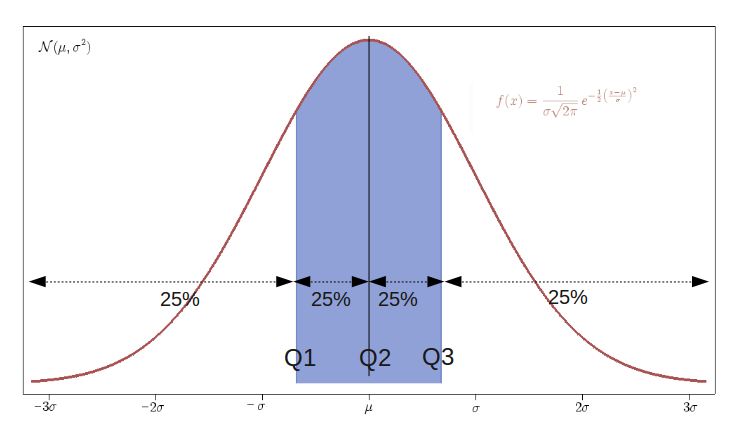
\includegraphics[scale=0.5]{secciones/consideraciones/imagenes/cuartiles.png}
\end{center}
\caption{Fuente: http://commons.wikimedia.org/wiki/File:Lqr\_with\_quantile.png}
\label{fig:cuariles}
\end{figure}

	Con el resto de los valores se realizó un promedio. Es muy importante notar que una vez eliminados los valores
atípicos la variación resulta realmente baja. En general de menos del 2\%. De esta manera se logra poder trabajar
con la media, que es una referencia muy fuerte, y además estar muy cerca del mínimo valor obtenido.

	

	

